
\documentclass[a4paper,12pt]{report}
\usepackage{graphicx}
\usepackage{url}
\begin{document}
\title{Maple Native Basic Test Procedures}
\author{LeafLabs}
\maketitle

\section*{}
\subsection*{1. Purpose of this Document}
This document provides basic setup and testing procedures for the LeafLabs Maple Native board. After following the procedures outlined in this document, basic functionality of the Maple Native board is guaranteed. The procedures in this document do not test full functionality of the Maple Native board, and additional testing is required before the board may be considered ``Quality Checked''.\\

You will need:

\begin{itemize}
\item a computer with all the required software
\item Mini-B USB cable
\item Serial-USB adapter (FTDI) with jumper wires to connect to Maple USART
\item a supply of header jumpers (2x per board)
\end{itemize}

\subsection*{2. Visual Inspection}

A brief visual inspection of the board should be performed to make sure there are no egregious physical errors. Some things to look out for are as follows:
\begin{itemize}
\item Is the silkscreen in focus/legible?
\item Are the buttons firmly in place? (Give them a nudge to be sure.)
\item Are there any visible shorts between pins?
\item Are there any large lumps of solder on any of the header?
\item Is there any un-melted solder paste?
\end{itemize}

\begin{center}
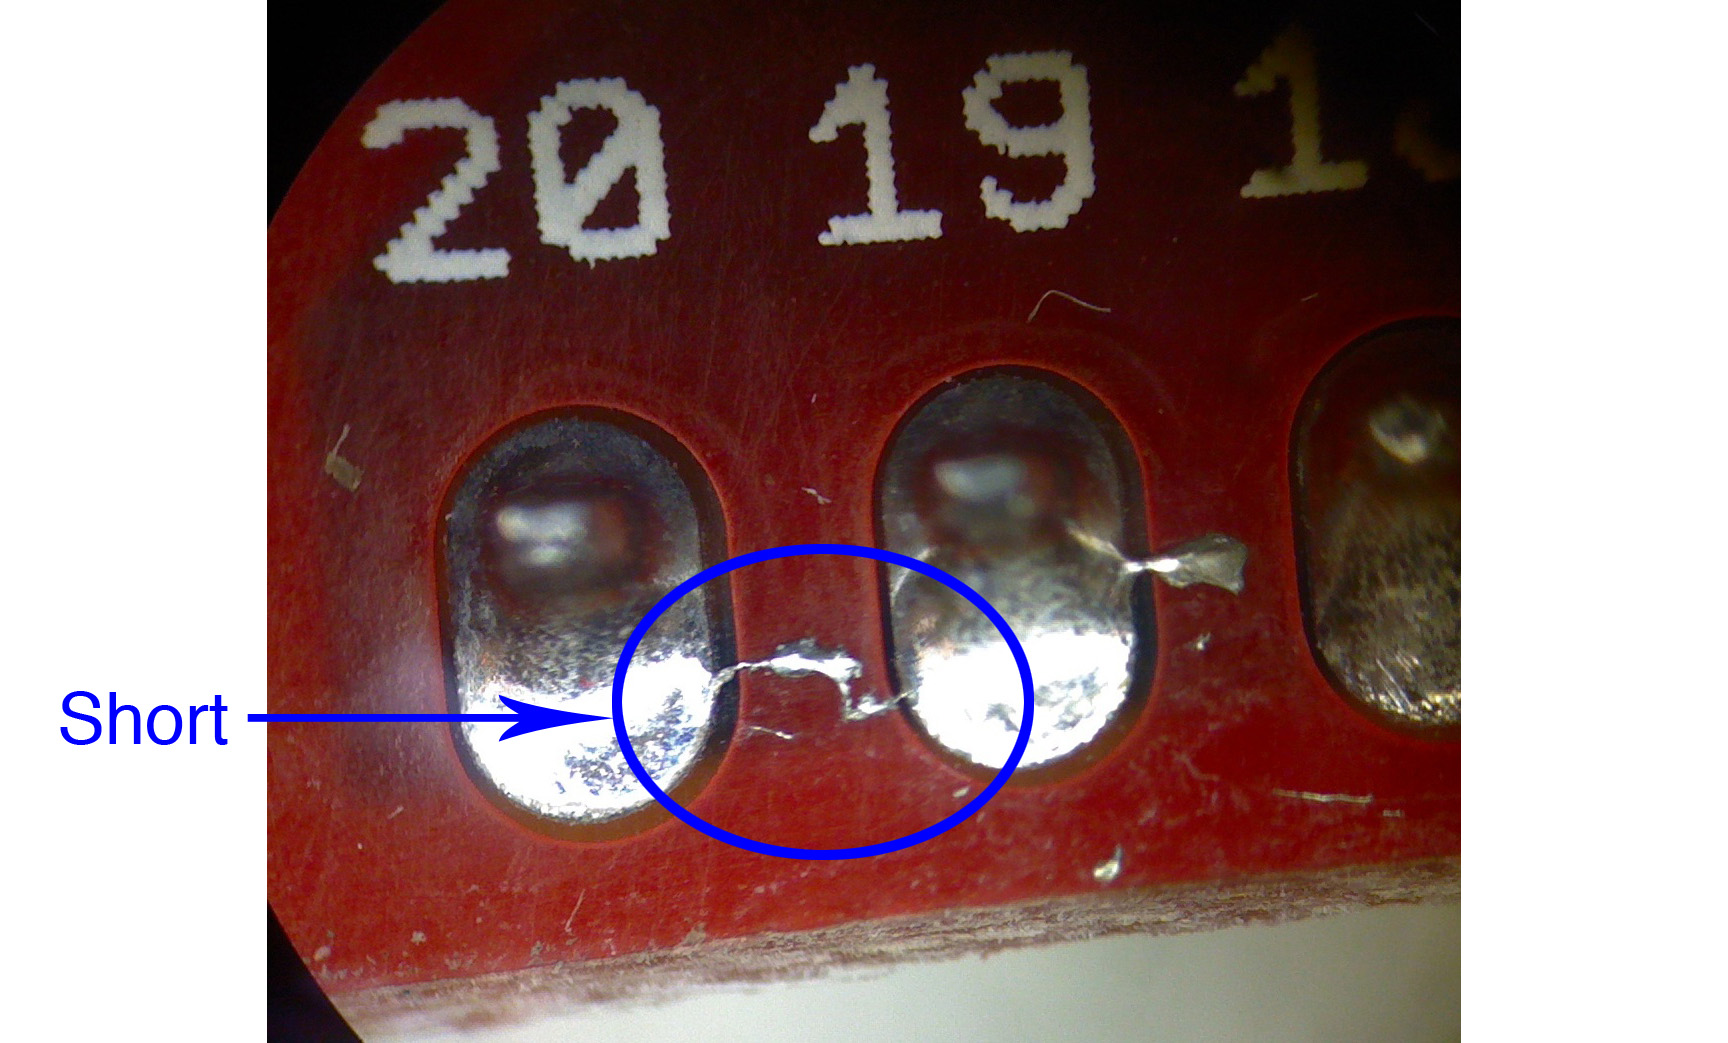
\includegraphics[width=\linewidth]{header-short}
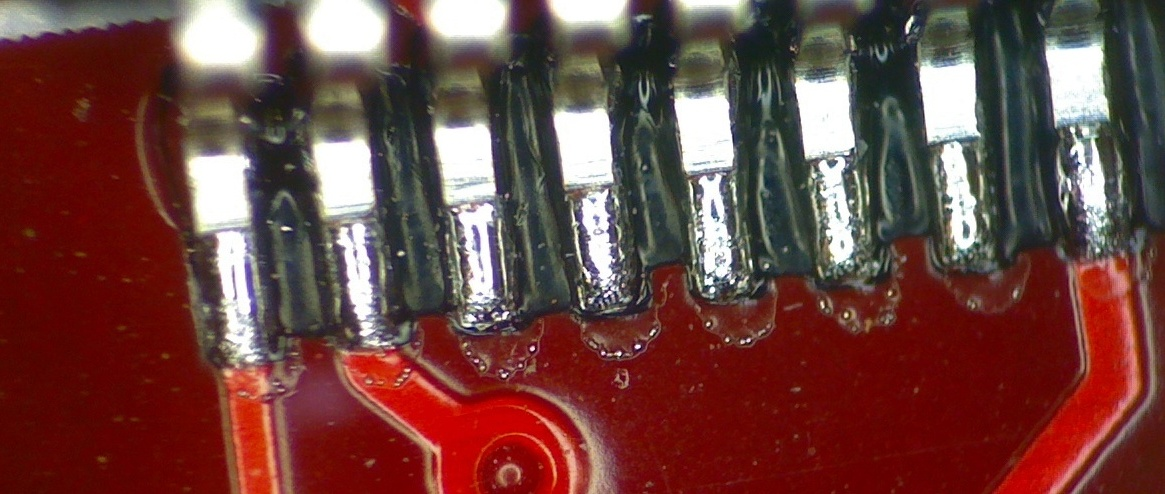
\includegraphics[width=\linewidth]{unmelted-solder}
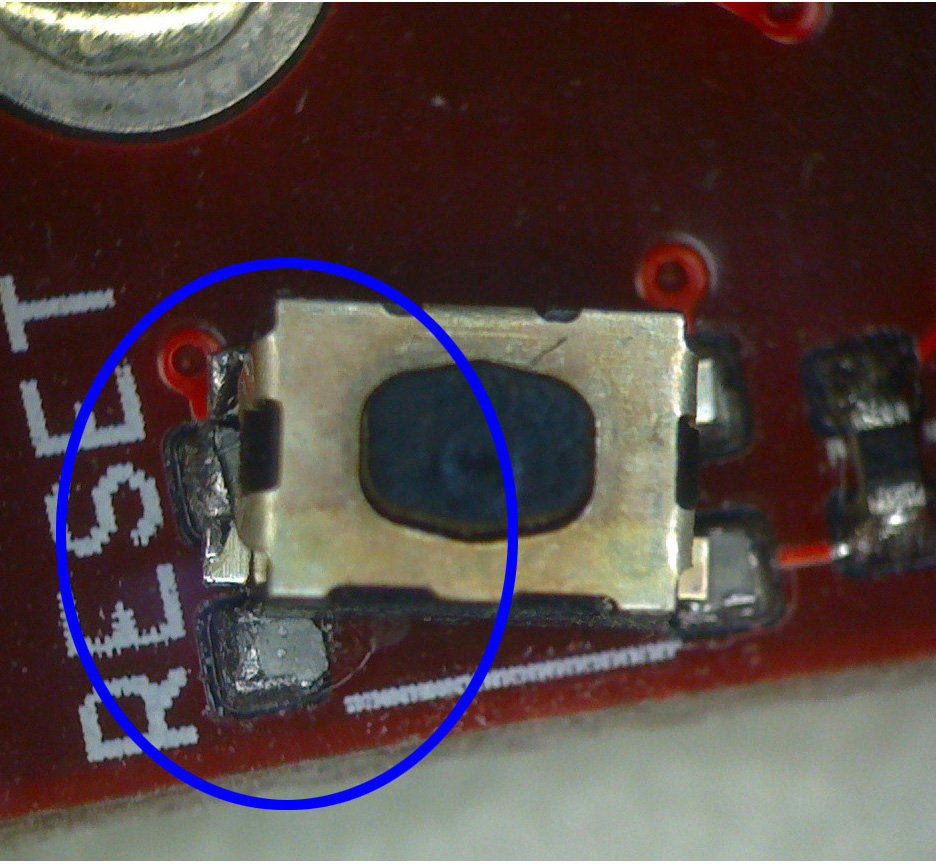
\includegraphics[width=\linewidth]{overheated-reset-button}
\end{center}

\subsection*{3. Attach Jumpers}

If the power select jumpers were not attached during production, they should be added at this stage. If they were attached, their proper placement should be verified. The power select jumper should be on USB and the battery charger should be half attached.

\begin{center}
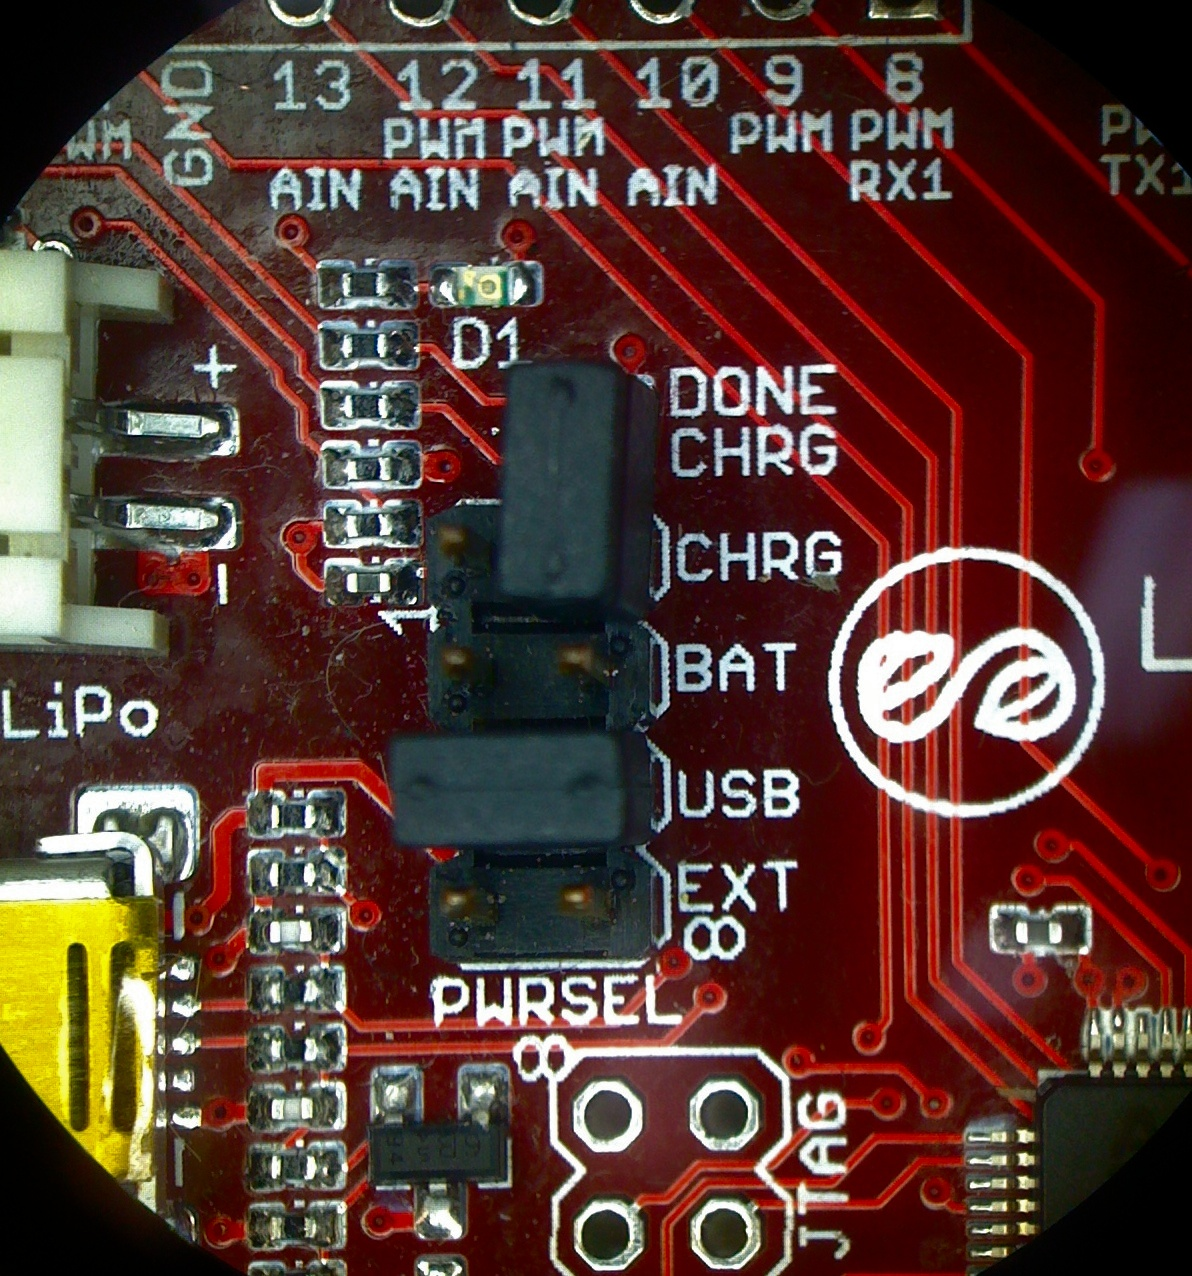
\includegraphics[width=\linewidth]{jumpers}
\end{center}

\subsection*{4. Flash bootloader}
The bootloader should be flashed via he hardware serial bootloader interface, as follows:

\begin{enumerate}
\item Download the stm32loader.py script from the \tt flash \rm directory of our maple-bootloader repository at \url{http://github.com/leaflabs/maple-bootloader}; this script (written by a third party) requires the PySerial library as well as a python runtime installed.
\item Get the most recent stable version of the bootloader from \url{http://static.leaflabs.com/pub/leaflabs/maple-bootloader/maple_native_boot.bin}
\item Connect both the FTDI chip and the Maple Native board to a computer via USB. Note that the Maple Native status light will not light up because there is no bootloader installed. 
\item Connect the FTDI chip to the Maple Native Serial1 USART device, which has TX1 on pin 24 and RX1 on pin 25. Be sure to connect Ground as well.
\item Ender hardware serial bootloader mode by pressing both the \tt BUT \rm and \tt RESET \rm buttons all the way down. Wait two seconds, then release \tt RESET. \rm Wait another two seconds, and release \tt BUT. \rm
\item Run the command \begin{verbatim}stm32loader.py -p /dev/ttyUSB0 -evw maple_native_boot.bin\end{verbatim} (note: this command assumes the FTDI chip is located at /dev/ttyUSB0; verify this beforehand and modify the command accordingly.) If the command runs successfully, there will be a long scroll of memory writes and verifications, then success. If the command does not run, it is possible the board did not successfully enter hardware bootloader mode. In this case, repeat steps 5 and 6 until success is achieved.
\item Press \tt RESET. \rm The blue status LED should blink perpetually.
\end{enumerate}

\subsection*{5. Upload test program}
To ensure basic functionality of the board, a test program must be uploaded, as follows:

\begin{enumerate}
\item Disconnect the FTDI chip from the computer and Maple Native. Leave Maple Native connected to the computer over USB.
\item Download and install the Maple IDE 0.0.10 Beta from \url{http://static.leaflabs.com/pub/leaflabs/maple-docs/0.0.10beta/maple-ide-install.html} (note: you \bf must \rm use 0.0.10 Beta; more recent versions will not work.
\item Open the Maple IDE and select Tools $\to$ Board $\to$ Maple Native (prototype) to Flash.
\item Select the appropriate serial port from Tools $\to$ Serial Port.
\item Open test program by selecting File $\to$ Examples $\to$ Digital $\to$ Blink.
\item Go to line 22 of the test program and change \begin{verbatim}int ledPin = 13;\end{verbatim} to\begin{verbatim}int ledPin = 22;\end{verbatim}
\item Click on the ``Upload'' button (second from the end) to upload the program.
\item The blue LED should now blink once per second. This, in addition to the message ``No error condition present. Done! Resetting USB switch back to runtime mode.'' from the IDE, indicates success.
\end{enumerate}

\end{document}

